\newpage
\section{Identification of Wave Spectrum Model}

In this section the Power Spectral Density (PSD) function, ${P_{{\psi _\omega }}}$ is covered.

%%%%%%%%%%%%%%%%%%%%%%%%%%%%%%%%%%%%%%%%%%%%%%%%%
% 2.1 Power Spectral Density Estimate
%%%%%%%%%%%%%%%%%%%%%%%%%%%%%%%%%%%%%%%%%%%%%%%%%
\subsection{Power Spectral Density Estimate, $S_{\psi_{\omega}}$}

A dataset with how waves have an impact on compass measurements is provided as a time series by ${\psi _\omega }$. To find an estimate for ${S_{{\psi _\omega }}}$ we use the following MatLab script with the function $[pxx, f] = ...pwelch(x, window, noverlap, nfft, fs)$ which utilizes discrete Fourier transform to estimate the PSD function from a time series signal. The function basically returns the two-sided Welch PSD estimates at the frequencies specified in the vector, f. 

\textbf{MatLab-script with \textit{pwelch}:}
\begin{lstlisting}
F_s = 10;
window = 4096;
noverlap = [];
nfft = [];  
[S_psi,f] = pwelch(psi_w(2,:).*(pi/180),window,noverlap,nfft,F_s);
omega = 2*pi.*f;
S_psi = S_psi./(2*pi);  
\end{lstlisting}

\begin{figure}[!htb]
    \caption{PSD Estimate, $S_{\psi_{\omega}}$}
    \centering
    \centerline{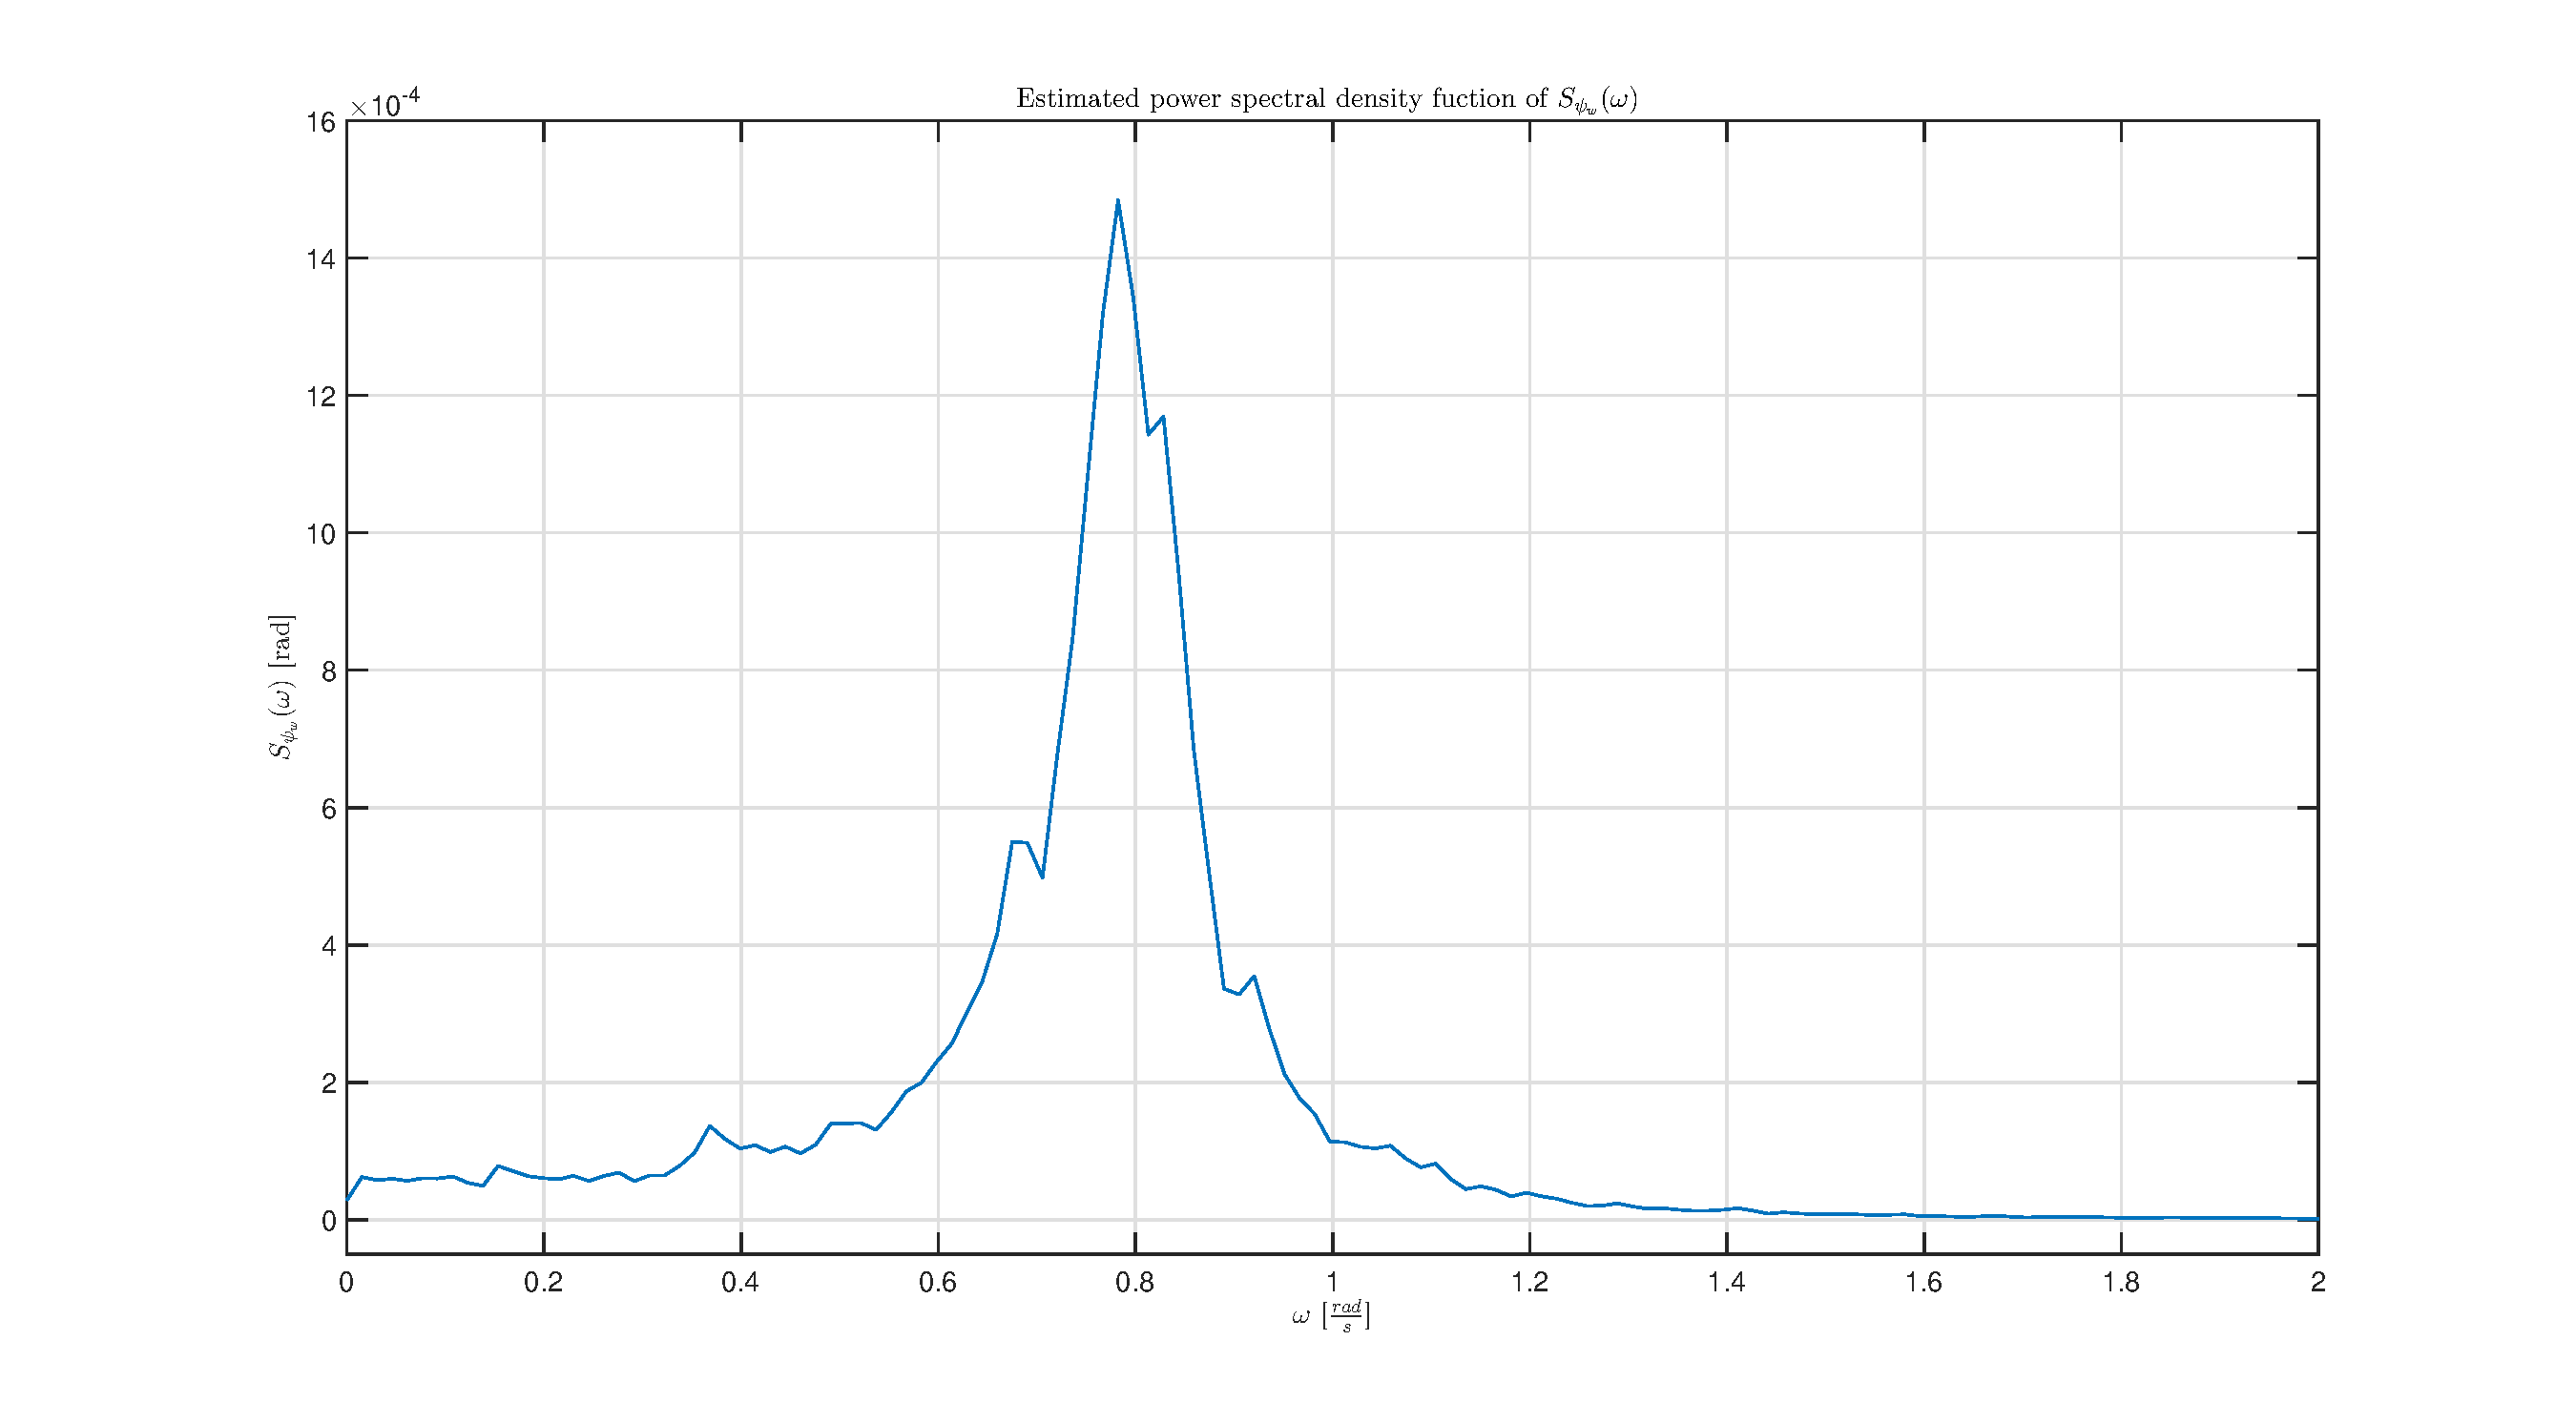
\includegraphics[scale=0.45]{plots/2a}}
    \label{plot:2a}
\end{figure}

%%%%%%%%%%%%%%%%%%%%%%%%%%%%%%%%%%%%%%%%%%%%%%%%%
% 2.2 Analytical Expressions for ${P_{{\psi _\omega }}}$ and ${H_{{\psi _\omega }}}$
%%%%%%%%%%%%%%%%%%%%%%%%%%%%%%%%%%%%%%%%%%%%%%%%%
\subsection{Analytical expressions for ${H_{{\psi _\omega }}}$ and ${P_{{\psi _\omega }}}$}

To obtain the transfer function ${H_{{\psi _\omega }}} = \frac{{{\psi _\omega }}}{{{\omega _\omega }}}$, which describes how the waves affect the yaw angle, we use the model (\ref{model}) as base.

\begin{align}\label{model}
    \begin{array}{l}
    {{\dot \xi }_w} = {\psi _\omega }\\
    {{\dot \psi }_\omega } =  - {\omega _0}^2{\xi _\omega } - 2\lambda {\omega _0}{\psi _\omega } + {K_\omega }{\omega _\omega }
\end{array}
\end{align}

Then Laplace transformation is applied to obtain the transfer function:

\begin{align*}
    \begin{array}{l}
        s\xi  = {\psi _\omega }\\
        s{\psi _\omega } =  - {\omega _0}^2{\xi _\omega } - 2\lambda {\omega _0}{\psi _\omega } + {K_\omega }{\omega _\omega }\\
        s{\psi _\omega } =  - {\omega _0}^2{\psi _\omega }\frac{1}{s} - 2\lambda {\omega _0}{\psi _\omega } + {K_\omega }{\omega _\omega }
\end{array}
\end{align*}

\begin{equation}
    {H_{{\psi _\omega }}} = \frac{{{\psi _\omega }}}{{{\omega _\omega }}} = \frac{{{K_\omega }s}}{{{s^2} + 2\lambda {\omega _0}s + {\omega _0}^2}}
\end{equation}

To find an analytical expression for ${P_{{\psi _\omega }}}$, we use the relationship expressed in (\ref{brown}). ${S_{{\omega _\omega }}}$ is defined by it being \textit{zero mean unity white noise}. This implies that the variance (${\sigma ^2}$) and spectral density (${S_{{\omega _\omega }}}$) are equal to 1.

\begin{equation}\label{brown}
    {P_{{\psi _\omega }}}(j\omega ) = {H_{{\psi _\omega }}}(j\omega ){H_{{\psi _\omega }}}( - j\omega ){S_{{\omega _\omega }}}
\end{equation}

\begin{equation}
    {P_{{\psi _\omega }}}(\omega ) = \frac{{{K_\omega }^2{\omega ^2}}}{{{\omega ^4} + 2(2{\lambda ^2} - 1){\omega _0}^2{\omega ^2} + {\omega _0}^4}}
\end{equation}


%%%%%%%%%%%%%%%%%%%%%%%%%%%%%%%%%%%%%%%%%%%%%%%%%
% 2.3 Finding $\omega_0$
%%%%%%%%%%%%%%%%%%%%%%%%%%%%%%%%%%%%%%%%%%%%%%%%%
\subsection{Finding $\omega_0$}

$\omega_0$ is the base frequency of the noise $\omega_\omega$ - the frequency which has the highest energy. Figure \ref{plot:2a} shows that is around $\frac{\pi}{4} rad/s$. To find the frequency which has the highest energy, the MatLab command \textit{[M, I] = max(A)}. The following MatLab-script were used to find $\omega_0$:

\textbf{Finding $\omega_0$:}
\begin{lstlisting}
[maxPSD, frequency_index] = max(S_psi);
omega_0 = omega(frequency_index);
\end{lstlisting}

Following values were obtained:

\begin{align*}
    \omega_0 &= 0.78233 \frac{{rad}}{s}\\
    \sigma^2 &= 4.8724 \frac{{\deg }}{{\frac{{rad}}{s}}}
\end{align*}



%%%%%%%%%%%%%%%%%%%%%%%%%%%%%%%%%%%%%%%%%%%%%%%%%
% 2.4 Identifying $\lambda$ and fitting $P_{\psi_\omega}$
%%%%%%%%%%%%%%%%%%%%%%%%%%%%%%%%%%%%%%%%%%%%%%%%%
\subsection{Identifying $\lambda$ and fitting $P_{\psi_\omega}$}

To identify the damping factor ($\lambda$), we use curve fitting. Some of the previous calculated values will be used in this identification where we use the MatLab command \textit{x = lsqcurvefit(fun, x0, xdata, ydata, lb, ub)}. \textit{lsqcurvefit} solves non-linear least squares problems. \textit{fun} is a function of \textit{x} and \textit{xdata} where the parameter(s) to be found is \textit{x} and \textit{xdata} is the abscissa data to fit into.

The following script provided $\lambda = 0.086198$.

\textbf{Finding $\lambda$ and $K_{\omega}$:}
\begin{lstlisting}
sigma = sqrt(maxPSD);
P_psi_fun = @(lambda,omega) ...
    (4*lambda^2*omega_0^2*sigma^2*omega.^2) ./ ...
    (omega.^4 + (2*lambda^2 - 1)*2*omega_0^2*omega.^2 + ...
    omega_0^4);

lambda0 = 10;
lb=0;
ub=10;
lambda = lsqcurvefit(P_psi_fun,lambda0,omega,S_psi,lb,ub);
K_w = 2*lambda*omega_0*maxPSD;
P_psi = P_psi_fun(lambda,omega);
\end{lstlisting}


\begin{figure}[!htb]
    \caption{Comparsion}
    \centering
    \centerline{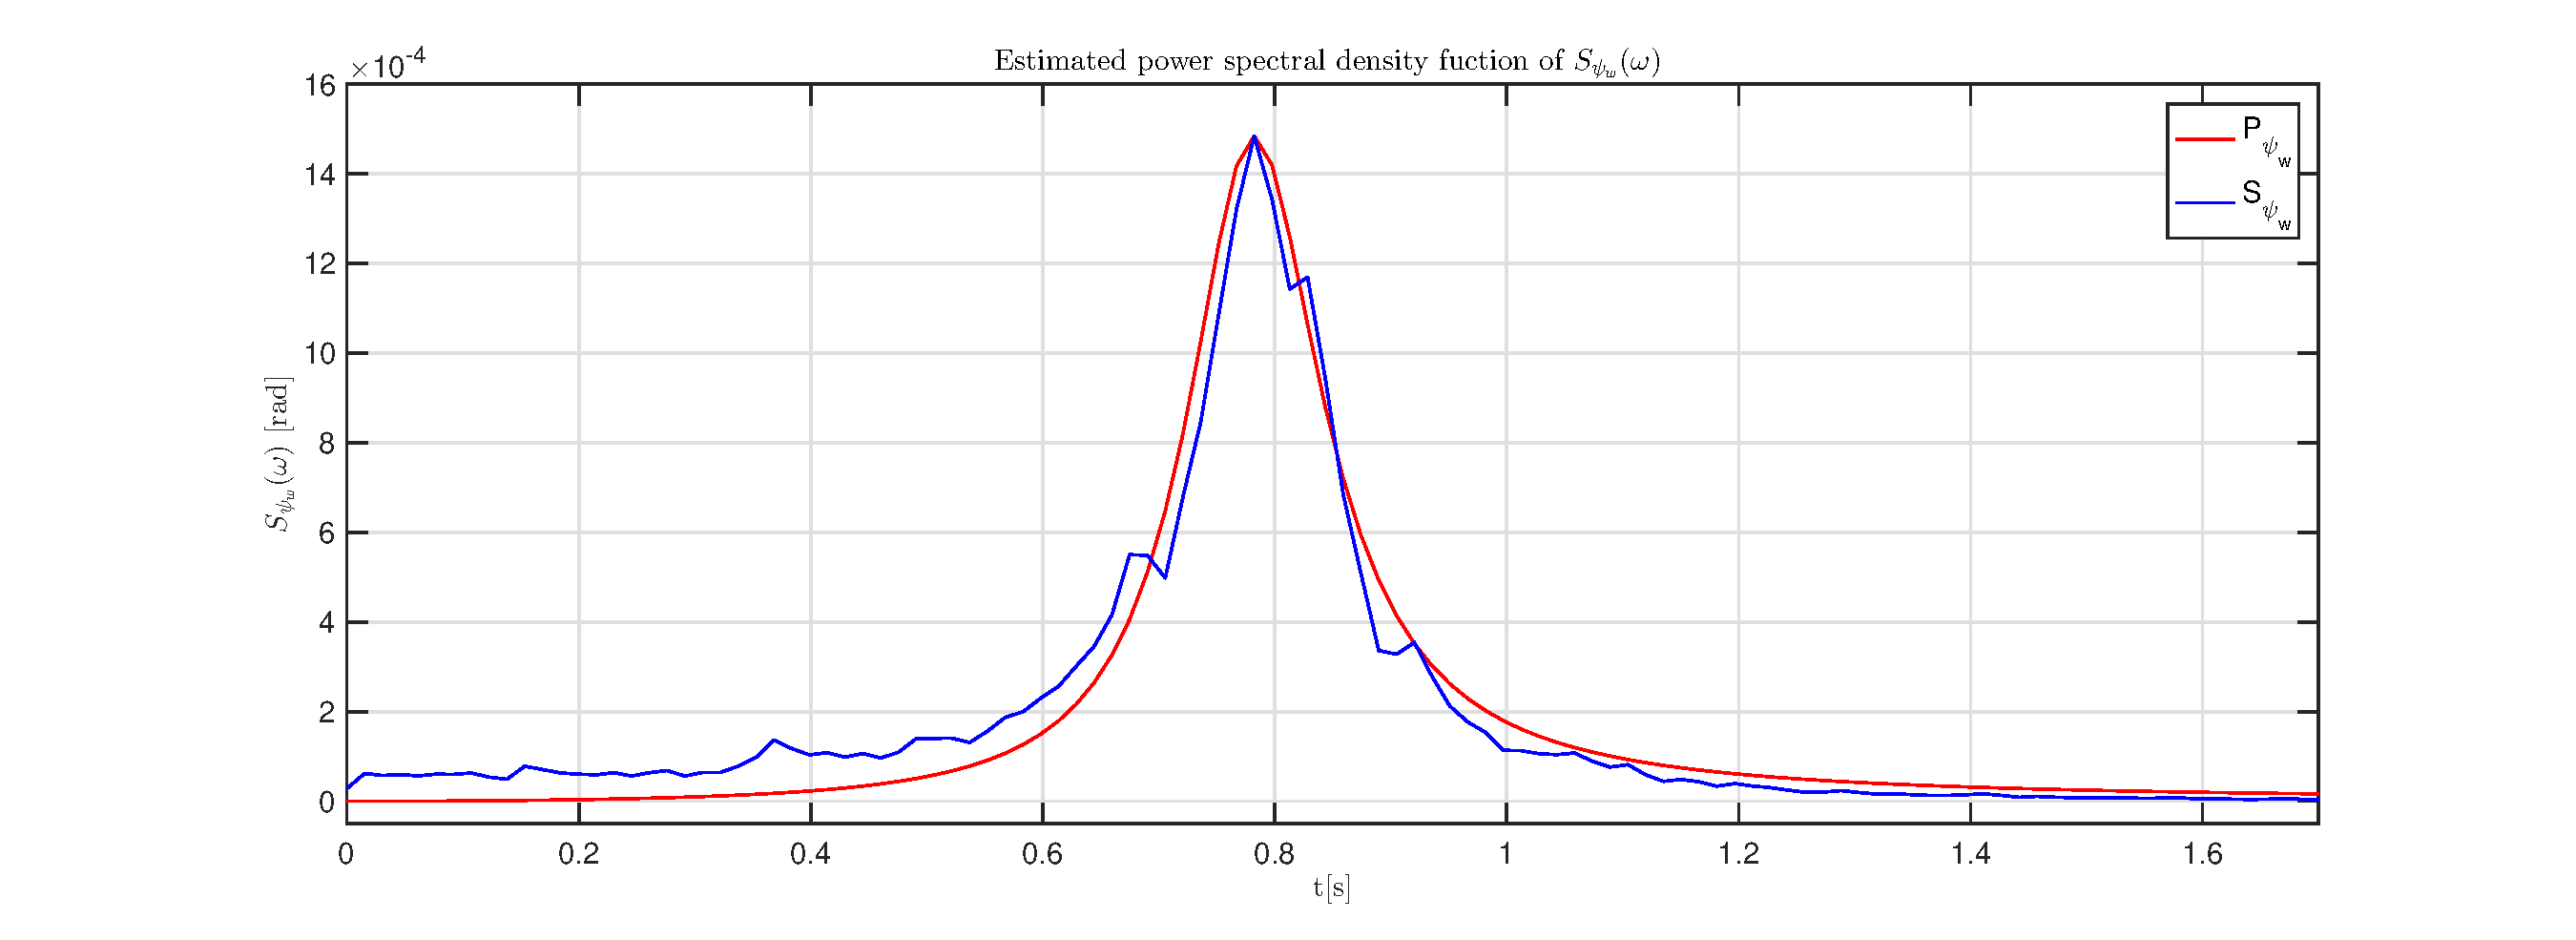
\includegraphics[scale=0.4]{plots/2d}}
\label{plot:2d}
\end{figure}

